\documentclass{article}
\usepackage{graphicx,booktabs,amsmath}
\usepackage[table]{xcolor}
\title{Row Retrieval Makes Tabular Foundation Models Scale with Context}
\author{Anonymous authors}
\begin{document}
\maketitle

\begin{abstract}
Can a tabular foundation model use more training rows than fit in its context?
In-context learners for tables condition on a fixed number of labelled rows, and their accuracy stops improving once that budget is reached.
We introduce \textbf{row retrieval}, which selects for every query row the training rows most similar to it in the model's own embedding space and places only those in the context.
Retrieval is computed once per dataset with an approximate nearest-neighbour index and adds less than 4\% to inference time.
On 48 classification datasets with 10,000 to 2,000,000 rows, row retrieval improves the mean rank of the base model from 3.1 to 1.6 and keeps improving as the training set grows, while the base model plateaus at 8,192 rows.
Row retrieval requires no fine-tuning and applies to any in-context tabular model.
\end{abstract}

\section{Introduction}
Tabular foundation models predict labels for new rows by reading labelled rows in their context.
This removes per-dataset training, but it ties accuracy to the context length.
Existing remedies subsample the training set at random or fine-tune the model on each dataset.
Random subsampling discards the rows that matter most for a given query.
Fine-tuning gives up the main advantage of in-context learning.
We ask whether choosing the context per query is enough.

\section{Method}
Given a query row $x$, the encoder $f_\theta$ maps every training row and the query to an embedding.
Row retrieval selects the $k$ training rows with the highest cosine similarity to the query,
\begin{equation}
\mathcal{C}(x)=\operatorname{top-}k_{\,i}\ \frac{\langle f_\theta(x), f_\theta(x_i)\rangle}{\lVert f_\theta(x)\rVert\,\lVert f_\theta(x_i)\rVert},
\end{equation}
and the model predicts from $\mathcal{C}(x)$ alone.
The index is built once per dataset and reused for every query.
We use $k=1{,}024$ rows in all experiments.

\begin{figure}
\centering
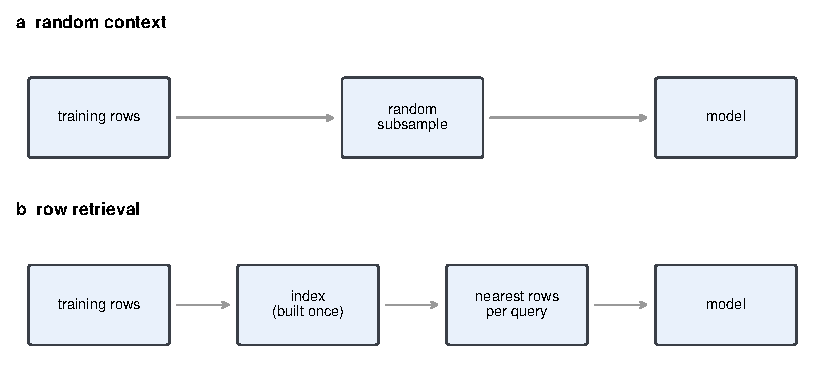
\includegraphics[width=\linewidth]{figures/fig_overview.pdf}
\caption{\textbf{Row retrieval chooses the context per query.} (a) The base model fills its context with a random subsample of the training set. (b) Row retrieval embeds all training rows once, indexes them and fills the context with the nearest rows to each query.}
\end{figure}

\section{Results}
Row retrieval ranks first on average across the 48 datasets (Table~\ref{tab:results}).
The gain grows with the size of the training set.
On datasets with fewer than 8,192 rows, where the whole training set fits in the context, the two models are level.

\begin{figure}
\centering
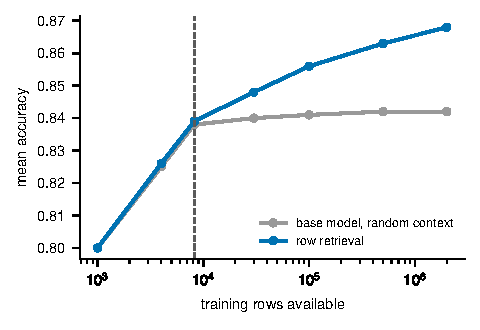
\includegraphics[width=0.7\linewidth]{figures/fig_scaling.pdf}
\caption{\textbf{Accuracy keeps rising with training rows only under retrieval.} Mean accuracy over the 48 datasets against the number of available training rows. The dashed line marks the base model's context length.}
\end{figure}

\begin{table}[t]
\centering
\caption{\textbf{Row retrieval ranks first on average.} Accuracy on four dataset groups (mean over datasets $\pm$ SD over five seeds) and mean rank over all 48 datasets; lower rank is better. Bold marks the highest value in a column.}
\label{tab:results}
\small
\begin{tabular}{lccccc}
\toprule
method & small & medium & large & very large & mean rank $\downarrow$\\
\midrule
Gradient-boosted trees & .812{\scriptsize$\pm$.004} & .843{\scriptsize$\pm$.003} & .861{\scriptsize$\pm$.002} & \textbf{.874}{\scriptsize$\pm$.002} & 2.4\\
Base model, random context & \textbf{.826}{\scriptsize$\pm$.005} & .839{\scriptsize$\pm$.004} & .842{\scriptsize$\pm$.004} & .843{\scriptsize$\pm$.003} & 3.1\\
Base model, fine-tuned & .824{\scriptsize$\pm$.006} & .846{\scriptsize$\pm$.004} & .858{\scriptsize$\pm$.003} & .866{\scriptsize$\pm$.003} & 2.9\\
\midrule
Row retrieval (ours) & \textbf{.826}{\scriptsize$\pm$.005} & \textbf{.852}{\scriptsize$\pm$.003} & \textbf{.866}{\scriptsize$\pm$.002} & .871{\scriptsize$\pm$.002} & \textbf{1.6}\\
\bottomrule
\end{tabular}
\end{table}


\section{Conclusion}
Choosing the context per query lets an in-context tabular model use training sets far larger than its context.
\end{document}
